
% This LaTeX was auto-generated from MATLAB code.
% To make changes, update the MATLAB code and republish this document.

\documentclass{article}
\usepackage{graphicx}
\usepackage{color}

\sloppy
\definecolor{lightgray}{gray}{0.5}
\setlength{\parindent}{0pt}

\begin{document}

    
    \begin{verbatim}
%Setup a pid controller

%CL RESPONSE     RISE TIME       OVERSHOOT  SETTLING TIME  S-S ERROR
%Kp              Decrease        Increase   Small Change   Decrease
%Ki              Decrease        Increase   Increase       Eliminate
%Kd              Small Change    Decrease   Decrease       No Change
clear all
clc

Kp = 1;     % 1 for a no change PID
Kd = 0;     % 0 for a no change PID
Ki = 0;     % 0 for a no change PID

Kc = 1;     % choose Kc = 1
Tl = 1;     % T for lead compensation
Tg = 0.05;  % T for lag compensation
A = 1;      % alpha (1 for no change to initial system)
B = 1;
Z=.5;

% stuff for S domain
s=tf('s');
GHs = (0.2*s +3.2)/((s+1)*(s+.8)); % plant
Gc = (s+1/Tg)/(s+1/(B*Tg)); % = 1 initially (lag)
Gl = (s+(1*A)/Tl)/(s+1/(Tl)); % = 1 initially (lead)
% setup the PID control
P = pid(Kp,Ki,Kd);

% stuff for solving
syms x b;
Px = Kp + Ki/x + Kd*x;              %pid
GHx = (0.2*x +3.2)/((x+1)*(x+.8));  % plant
\end{verbatim}
\begin{par}
design a lag controller pick Kc=1 find Kv
\end{par} \vspace{1em}
\begin{verbatim}
Cg = (x+1/Tg)/(x+1/(b*Tg));         % lag
kc = limit((x * Cg * Px * GHx),0);

% set Beta to that value so Kv=5
if kc==0
    B=1;
else
    B = double(solve(kc==5,b));
end


%setup the lag compensator using B found above
Cg = (x+1/Tg)/(x+1/(B*Tg));     % lag
limit((x * Cg * Px * GHx),0)
Kv = limit((x * Cg * Px * GHx),x,0);
\end{verbatim}

        \color{lightgray} \begin{verbatim} 
ans =
 
0
 
\end{verbatim} \color{black}
    \begin{par}
Design a lead controller
\end{par} \vspace{1em}
\begin{verbatim}
%setup the lead compensator using A found above

Cl = (x+(1*A)/Tl)/(x+1/(Tl));    % lead

limit((x * Cg * Px * GHx),0)
Kl = limit((x * Cg * Cl * Px * GHx),x,0);
\end{verbatim}

        \color{lightgray} \begin{verbatim} 
ans =
 
0
 
\end{verbatim} \color{black}
    \begin{verbatim}
% show root locus
figure()
rlocus(P * Kc * Gc * Gl * GHs)
hold on
rlocus(GHs)
sgrid
hold off
figure()
sys = feedback(P * Kc * Gc * Gl * GHs,1);

% show unit step plot
step(sys)
t = 0:.01:100;
figure()
% show unit ramp plot
lsim(sys,t,t)
title('Response to Unit Ramp Input')
sse = abs(1-dcgain(sys));
S = stepinfo(sys);

tf(P * Kc * Gc * Gl * GHs)
fprintf('For the new system shown above the following results. \n');
fprintf('The sse is %f\n',sse);
fprintf('The overshoot is %f\n',S.Overshoot);
fprintf('The settling time is %f\n',S.SettlingTime);
fprintf('The value of Kv is %s\n',char(Kv));
\end{verbatim}

        \color{lightgray} \begin{verbatim}
ans =
 
      0.2 s^3 + 7.4 s^2 + 71.2 s + 64
  ---------------------------------------
  s^4 + 22.8 s^3 + 58.6 s^2 + 52.8 s + 16
 
Continuous-time transfer function.

For the new system shown above the following results. 
The sse is 0.200000
The overshoot is 16.441601
The settling time is 3.977884
The value of Kv is 0
\end{verbatim} \color{black}
    
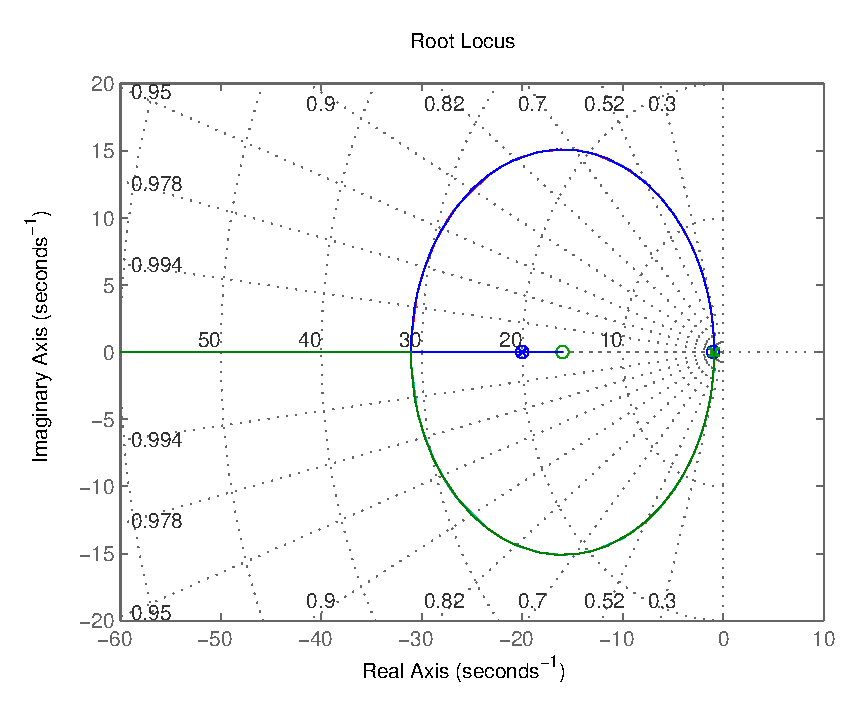
\includegraphics [width=4in]{EEL3657_01.eps}

\includegraphics [width=4in]{EEL3657_02.eps}

\includegraphics [width=4in]{EEL3657_03.eps}



\end{document}
    
